\section{Gravitationally unstable disks} \label{result2}
Gravitational instability becomes possible in a sufficiently
massive and/or cold disk. Here, we explore whether or not GI and MRI
can interact by computing unstable modes for isothermal disks with $Q < 0.2 $
($Q_\mathrm{2D}\lesssim ~0.67$) which permits GI, as shown below.
We consider ideal disks with $\Lambda_0=100$ and $A=1$, unless
otherwise stated.  

\subsection{Co-existence of MRI and GI} 
Fig. \ref{compare_growth3} show growth rates for modes with $k_xH=1$
as a function of $\beta$ in disks with $Q=0.18$, $Q=0.14$ and
$Q=0.12$.   
All three cases display distinct GI modes (red/brown branch). The GI 
growth rates are $\gamma\simeq 0.25\Omega,\,0.6\Omega,\,0.8\Omega$ for
$Q=0.18,\,0.14,\,0.12$, respectively. GI is stabilized by magnetic
pressure for sufficiently small $\beta$. The critical
field strength for stabilizing GI increases with increasing
self-gravity, consistent with \cite{nakamura83}.   
For $Q=0.18$, GI is stabilized for $\beta \lesssim 15$. Nevertheless, 
the MRI branch for $\beta < 15$ becomes self-gravitating, so that
density perturbations still grow, even though GI does not
formally operate.  

%critical beta increases with $Q$

\begin{figure}
  \includegraphics[width=\linewidth,clip=true,trim=0cm 2.1cm 0cm
    0cm]{figures/compare_growth3_kx1_Q0d18.ps} 
  \includegraphics[width=\linewidth,clip=true,trim=0cm 2.1cm 0cm
    0.5cm]{figures/compare_growth3_kx1_Q0d14.ps} 
  \includegraphics[width=\linewidth,clip=true,trim=0cm 0cm 0cm
    0.5cm]{figures/compare_growth3_kx1_Q0d12.ps} 
  \caption{Growth rates for modes with $k_xH=1$ in isothermal ideal
    disks with $Q=0.18$ (top), $Q=0.14$ (middle) and $Q=0.12$ (bottom). The
    colorbar measures the importance of  
    self-gravity by $\tau$.   
    \label{compare_growth3}}
\end{figure}

The GI and MRI branches only interact when their growth rates
are similar. This is seen in Fig. \ref{compare_growth3} for $Q=~0.18$
where the GI branch approaches a MRI branch at $\beta\simeq 25,\,
\gamma\simeq 0.2\Omega$. In fact, following the red curve to smaller
$\beta$ indicates GI transitions to MRI. The
`gaps' in the GI and MRI branches for $Q=0.18$ and $Q=0.12$ may be due
to the phenomenon of avoided crossing, as seen in stars
\citep[e.g.][]{aizenman77} and accretion tori
\citep[e.g.][]{christo93}, where physically distinct modes approach
one another in frequency and exchange character. However, we cannot
exclude the possibility  that some modes may have been missed in a 
numerical search of eigenfrequencies.  
%maybe ogilvie?

Thus, our results do not rigorously prove that the GI and MRI branches
do not intersect.  Nevertheless, the continuous variation of $\tau$
strongly suggest that unstable modes can transition smoothly from 
MRI to GI and vice versa, especially at low $\beta$.     
%no unique transition

\subsubsection{Case study} 
In reality, perturbations with a range of $k_x$ will be present for a
given set of disk parameters. Fig. \ref{compare_growth3_Q01d2} show
growth rates as a function of $k_x$ in a disk with
$Q=0.12,\,\beta=20$, where MRI and GI have comparable growth
rates. All perturbations with $k_xH \lesssim 3.5$ grow dynamically
($\gamma\gtrsim 0.1\Omega$, or $\lesssim$ 1.6 orbits).

We also plot in Fig. \ref{compare_growth3_Q01d2} growth rates obtained 
from the Cowling approximation, which isolates MRI; and that from a
high-resistivity run, which isolates GI by allowing the field lines to
slip through the fluid. We refer to these as  
pure MRI and pure GI, respectively.  
For $k_xH\lesssim 0.7$, growth rates are equal to
those on the pure MRI and pure GI branches. That is, MRI and GI
operate independently until their growth rates become equal as a
function of $k_x$.  

The dispersion relation $\gamma(k_x)$ deviates from the
pure GI/MRI curves with increasing $k_x$, implying stronger interaction between
magnetic and density perturbations. Comparing pure GI (dashed line)
and the gravitationally-dominated portions of $\gamma(k_x)$ shows that 
inclusion of magnetic field stabilizes high-$k_x$ pure GI. (Note also
the slight decrease in the most unstable $k_x$.) 
This stabilization is due to magnetic pressure \citep{lizano10}, which
is consistent with stabilizing the small wavelength GI only.    

Comparing pure MRI (solid line) and the magnetically-dominated
portions of $\gamma(k_x)$ show that self-gravity increases MRI growth
rates at large $k_x$. This effect is small but noticeable, which can
be used as a code test for non-linear simulations. Note that this
destabilization is through the linear response, rather 
than through the background stratification (which is stabilizing).  

%smooth transitions, mode exchange

\begin{figure}
  \includegraphics[width=\linewidth]{figures/compare_growth3_Q0d12_B20.ps}  
  \caption{Growth rates of unstable modes in the massive isothermal
    disk with $Q=0.12$ and $\beta=20$, as a function of the horizontal
    wavenumber $k_x$. The colorbar measures the importance of
    self-gravity by $\tau$. The solid line corresponds to MRI modes in the
    Cowling approximation. The dashed line corresponds to pure GI
    modes, obtained by including a high resistivity in the full
    problem. 
    \label{compare_growth3_Q01d2}}
\end{figure}

